\chapter{Introdução}

A introdução eu devo escrever por último, deve conter a importancia do projeto, devo descrever o problema e a solução: "existe um problema e foi resolvido assim". O final da introdução deve descrever a estrutura dos capitulos dando uma pincelada rapida em cada um.

\chapter{Conceitos}
\section{Arquitetura de Software}
\section{Atributos de Modularidade}
\subsection{Acoplamento}
\subsection{Coesão}

\chapter{Implementação do Extrator}

O projeto consiste na implementação de um novo extrator para o egypt onde a análise seja feita direto do código fonte do projeto sem necessidade de compilação, ou seja, o novo extrator irá buscar as informações diretamente no código fonte sem necessidade de compilação, seja pelo GCC ou outro compilador qualquer. Isto trará duas vantagens imediatas, primeiro: será possível analisar projetos que não compilem mais, seja por falhas no código fonte ou por possuir dependencias não satisfeitas e segundo: a análise de um projeto irá levar menos tempo do que com o extrator atual (isto precisa ser testado).

\section{egypt}

O egypt foi originalmente desenvolvido por Andreas Gustafsson\footnote{http://www.gson.org/egypt} com o objetivo de gerar gráficos de chamada entre funções de programas escrito em C, ele funciona lendo os arquivos intermediários gerados pelo GCC\sigla{GCC}{GNU C Compiler} e os converte num gráfico de chamada no formato usado pelo Graphviz\footnote{http://www.graphviz.org}, um programa para visualização de gráficos.

O egypt é Software Livre e em Janeiro de 2009 começou a ser restruturado por Antonio A S. Terceiro o qual o tem mantido em\footnote{http://github.com/terceiro/egypt}. As principais mudanças sofridas pelo egypt deste então foram \cite{StructuralComplexityEvolution}:

\begin{itemize}
\item Detecção de uso de variáveis, para identificar que função usa qual variável.
\item Opção para agrupar chamada e uso de variaveis por módulo, com isto é possível ter uma visão de dependência entre módulos.
\item Refatoração do script egypt em um design orientado a objetos, para permitir diferentes módulos de extração e relatório.
\item Geração de relatório de métricas, como coesão e acoplamento.
\end{itemize}

\section{Doxygen (e a sua API)}

Doxygen\footnote{http://www.doxygen.org} é um sistema de documentação para C, C++, Java, Python e outros. Com ele é possível gerar documentação em HTML, RTF, PostScript, PDF e man pages, ele extrai a documentação explícita escrita pelo programador em comentários no código fonte seguindo uma sintaxe própria, e também tem a capacidade de extrair diretamente do código fonte informações de hierarquia e colaboração entre as classes. É baseado nesta capacidade de extrair informações do código fonte diretamente que o Doxygen foi escolhido como base para implementação deste novo extrator para o egypt.

O Doxygen é Software Livre e está disponível sob a GPL \sigla{GPL}{GNU Public License} em \footnote{https://doxygen.svn.sourceforge.net/svnroot/doxygen/trunk}, junto ao código fonte do projeto existe um exemplo chamado doxyapp de uma ferramenta para parsing de código fonte bem próximo as necessidades deste projeto.

Entre as inúmeras classes presentes na API do Doxygen é importante destacar as clasess: Doxygen, CodeOutputInterface, MemberDef e FileDef.

\begin{itemize}
\item Doxygen - Esta classe provê um namespace para varáveis e funções globais usadas pelo doxygen
\item CodeOutputInterface - Interface de saída para os parsers de código fonte
\item MemberDef - Definição de um membro (símbolos) de classe
\item FileDef - Definição de um arquivo
\end{itemize}

Este exemplo implementa a interface CodeOutputInterface da API do Doxygen, este interface serve para quem deseja escrever trecho de código extraido do código fonte do projeto na documentação gerada pelo Doxygen. Seguindo esta interface é possível implementar um parser reaproveitando todo o poder que o Doxygen fornece para análise de código fonte e gerar a saída da forma desejada.



\section{Implementação do Extrator usando a API do Doxygen}

O Doxygen apesar de oferecer todos os recursos básicos necessários para analisar um código fonte em C/C++ e extrair o uso de símbolos (funções, varáveis, etc) não faz o trabalho de simplesmente extrair estes dados sem gerar saída em PDF ou RTF por exemplo.


Neste projeto foi implementado uma ferramenta chamado doxyparse seguindo esta interface onde são definidos parametros para o Doxygen deacordo com as nossas necessidades como por exemplo: analisar o diretorio recursivamente, não gerar saida em Latex ou HTML, extrair tant informação quanto possível do codigo fonte, gerar gráfico de chamada, etc.

Este parser então faz a análise dos fontes de um diretorio passado via linha de comando e extrai destes fontes os simbolos encontrados onde são definidos e onde são usados/chamados. Com isto em mão ele gera uma saída num formato convinente para ser depois analisado pelo extrator implementado no egypt. Exemplo de saída gerado pelo doxyparse:

\begin{verbatim}
module module1.c
   function main in line 5
      uses function callback defined in module3.c
      uses function say_bye defined in module2.c
      uses function say_hello defined in module2.c
      uses variable variable defined in module3.c
\end{verbatim}

Com a saída gerada pelo doxyparse em mãos o egypt precisa agora de um extrator que entenda estes dados e armazene as informações encontradas para então depois gerar a saída para o Graphviz gerar o gráfico ou para gerar as métricas implementadas no egypt. Como o egypt já tem uma infraestrutura para possibilitar novos extratores não foi difícil criar um novo, o egypt possui uma classe chamada Extractor que representa extrator baseado nos arquivos intermediários do GCC, este classe foi transformada numa implementação de extrator genérica contendo apenas uma interface para cada extrator especifico implmentar e foi criado inicialmente 2 estratores, o GCC baseado no código já existente e o Doxyparse um novo extrator que usa como entrada os dados gerados pelo doxyparse baseado no Doxygen.

\begin{figure}[h]
\center
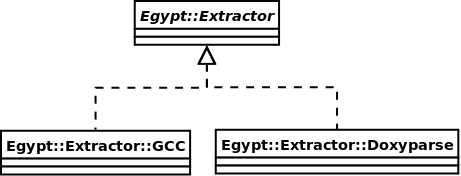
\includegraphics[scale=0.5]{imagens/egypt-diagram-extractor}
\label{egypt-diagram-extractor}
\caption{diagrama da hierarquia de classes do extrator do egypt}
\end{figure}

\chapter{Avaliação}

Nos resultados eu posso comparar o que consegui com a nova ferramenta comparado ao modo antigo do egypt extrair informacoes.

\section{Procedimento}

Primeiro foi feito um estudo sobre o Doxygen para entender seu funcionamento e verificar a viabilidade de usá-lo, então implementou-se o doxyparse baseado no exemplo vindo junto ao doxygen, a partir daí o egypt foi alterado para permitir a implementação do extrator baseado no doxyparse e entao foi implementado o Egypt::Extractor::Doxyparse.

Com o extrator Doxyparse pronto, inicia-se a etapa de extração de informações do projeto de softwalire ristretto,um software livre escrito em C para visualização de imagens, este projeto foi utilizado por Antonio Terceiro para o experimento X (fonte?) onde foi gerado dados de dependencia entre módulos para as versões 0.0.1 até a 0.0.21 deste projeto. Foi gerado os mesmos dados utilizando o extrator Doxyparse e então comparados aos dados extraidos pelo extrator GCC.

\section{Resultados}

Os resultados obtidos foram satisfatórios e atingiram o objetivo inicial que foi possibilitar estração de dados sem necessidade de compilar o software em questão, contudo algumas diferenças entre o extrator original do egypt e o atual baseado no Doxyparse foram notadodas. Nas Figuras \ref{ristretto-0.0.1}, \ref{ristretto-0.0.11} e \ref{ristretto-0.0.21} estão gráficos de chamadas entre módulos das versões 0.0.1, 0.0.11 e 0.0.21 do ristretto gerado pelo egypt usando o extrator Doxyparse e o GCC :

\begin{figure}
\center
\subfigure[ristretto-0.0.1-doxyparse][Egypt::Extrator::Doxyparse]{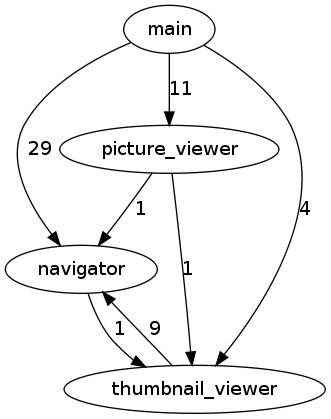
\includegraphics[scale=0.5]{imagens/ristretto-0_0_1-doxyparse}}
\qquad
\subfigure[ristretto-0.0.1-gcc][Egypt::Extrator::GCC]{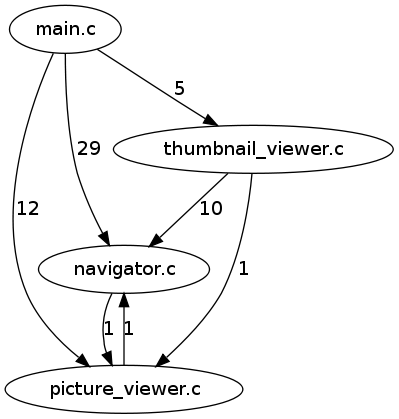
\includegraphics[scale=0.5]{imagens/ristretto-0_0_1-gcc}}
\caption{gráfico de chamada entre módulos do {\bf Ristretto 0.0.1} gerado pelo Egypt}
\label{ristretto-0.0.1}
\end{figure}

Na Figura \ref{ristretto-0.0.1} nota-se uma diferença interessante entre as informaçõe extraídas pelo GCC e Doxyparse, há uma inversão entre os módulos thumbnailer\_viewer e picture\_viewer. Enquanto o Doxyparse diz que o picture\_viewer chama o thumbnailer\_viewer no GCC temos o contrário, qual deles está errado ou os dois estão errados?

\begin{figure}
\center
\subfigure[ristretto-0.0.11-doxyparse][Egypt::Extrator::Doxyparse]{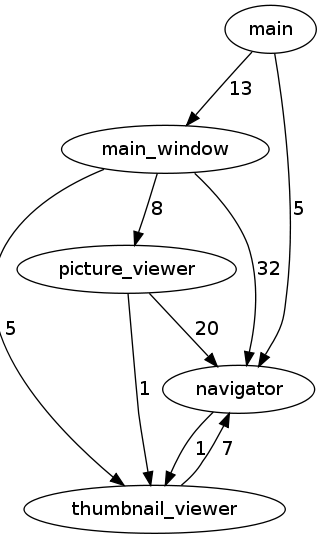
\includegraphics[scale=0.5]{imagens/ristretto-0_0_11-doxyparse}}
\qquad
\subfigure[ristretto-0.0.11-gcc][Egypt::Extrator::GCC]{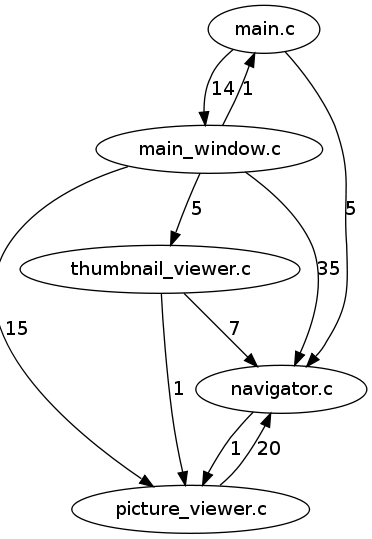
\includegraphics[scale=0.5]{imagens/ristretto-0_0_11-gcc}}
\caption{gráfico de chamada entre módulos do {\bf Ristretto 0.0.11} gerado pelo Egypt}
\label{ristretto-0.0.11}
\end{figure}

O mesmo ocorre nas Figuras \ref{ristretto-0.0.11} e \ref{ristretto-0.0.21}, mas nestas outras ainda temos mais observações, por exemplo na Figuras \ref{ristretto-0.0.11} o GCC diz que o módulo main\_window chama main, já no Doxyparse não há esta chamada.

\begin{figure}
\center
\subfigure[ristretto-0.0.21-doxyparse][Egypt::Extrator::Doxyparse]{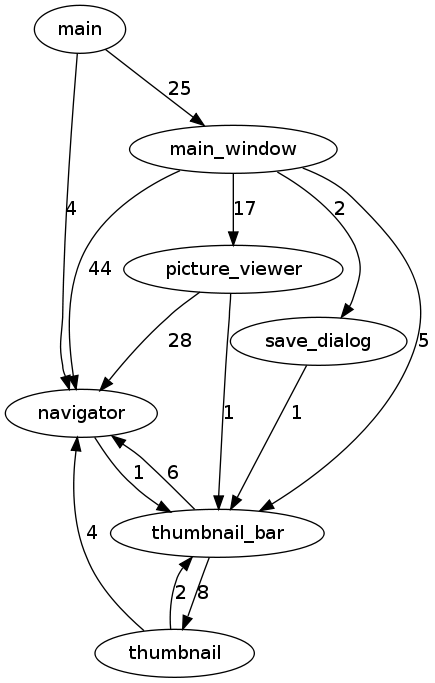
\includegraphics[scale=0.5]{imagens/ristretto-0_0_21-doxyparse}}
\qquad
\subfigure[ristretto-0.0.21-gcc][Egypt::Extrator::GCC]{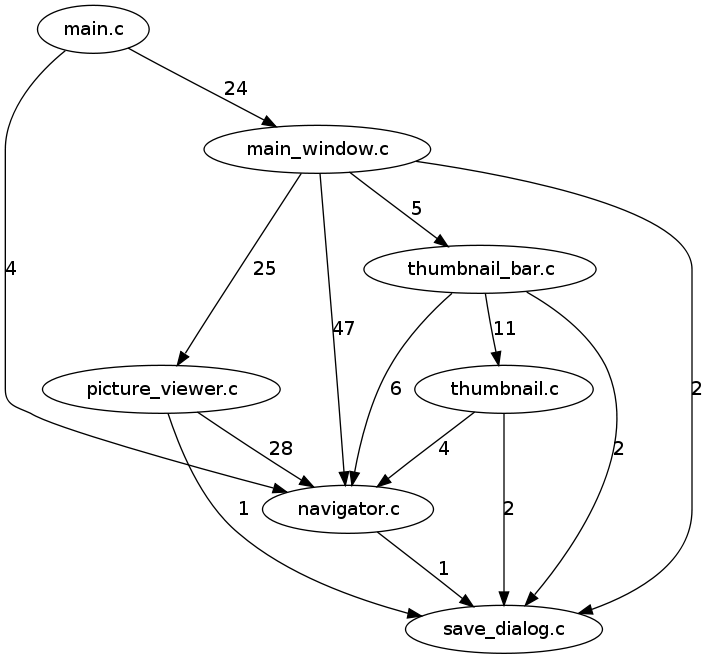
\includegraphics[scale=0.5]{imagens/ristretto-0_0_21-gcc}}
\caption{gráfico de chamada entre módulos do {\bf Ristretto 0.0.21} gerado pelo Egypt}
\label{ristretto-0.0.21}
\end{figure}

Na Figura \ref{ristretto-0.0.21} temos ainda outra importante, o GCC nos diz que o módulo save\_dialog é chamado por vários módulos: main\_window, thumbnail, navigator, picture\_viewer e thumbnail\_bar sendo que não faz sentido já que este é um módulo que encapsula a exibição de uma caixa de diálogo onde teoricamente deveria ser chamada apenas pelos módulos que compõe a interface, como diz o Doxyparse que apenas main\_window chama save\_dialog, mas o Doxyparse dá uma informação controversa onde o save\_dialog chama thumbnail\_bar e isto pode não ser verdade (verificar).

\section{Discussão}

\chapter{Conclusão}

A conclusão eu devo escrever por último, deve conter algo assim: "Este trabalho tinha objetivo tal e atingiu tal objetivo". Deve ter referencia de como foi feito e se os resultados foram bons, medios, satisfatorios, ruins, etc. E ao final deve ter trabalhos futuros que eu tenha interesse ou não de fazer.

Trabalhos futuros: verificar Natural Docs, semelhando ao Doxygen implementado em Perl e suporta outras linguagens.
